\section{Interfejs graficzny}

\begin{center}
	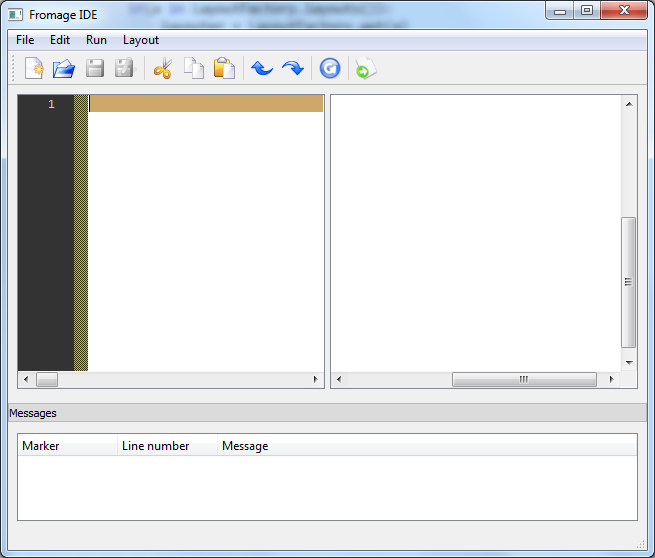
\includegraphics[width=0.66\textwidth]{fromage_ide}
\end{center}

Po uruchomieniu programu powinniśmy zobaczyć okno główne składające się z trzech paneli:

\begin{itemize}
	\item Edytor - panel służący do edycji aktualnie otwartego dokumentu.
	\item Podgląd - panel podglądu diagramu
	\item Lista błędów - sygnalizująca błędy w dokumencie
\end{itemize}

\subsection{Pasek menu oraz pasek narzędzi}
Opcje programu można wywoływać poprzez ikony na pasku narzędzi lub poprzez pasek menu.

Kolejno na pasku narzędzi znajdują się:
\begin{itemize}
	\item ,,New'' - otwiera nowy (pusty) dokument
	\item ,,Open document'' - otwiera istniejący dokument
	\item ,,Save'' - zapisuje aktualnie otwarty dokument
	\item ,,Save as'' - umożliwia zapisanie aktualnie otwartego dokumentu z wyborem nowej nazwy
	\item ,,Cut'' - funkcja ,,wytnij''
	\item ,,Copy'' - funkcja ,,kopiuj''
	\item ,,Paste'' - funkcja ,,wklej''
	\item ,,Undo'', ,,Redo'' - ,,cofnij'', ,,potwórz''
	\item ,,Generate'' - generuje diagram i wyświetla go w panelu podglądu
	\item ,,Export'' - zapisuje diagram widoczny w panelu podglądu do pliku obrazka
\end{itemize}

Dodatkowo na pasku menu znajduje się kategoria ,,Layout''. Menu ,,Layout'' służy do wyboru algorytmu rozkładania diagramów przy generacji. Do wyboru są różne algorytmy, zaleznie od platformy (a mianowicie obecności biblioteki \textbf{graphviz}).

\subsection{Praca z programem}

Zazwyczaj praca z programem rozpoczyna odczytania istniejącego dokumentu lub rozpoczęcia pracy nad nowym dokumentem - w drugim przypadku można zacząć pracować na pustym dokumencie który jest dostępny odrazu po otwarciu aplikacji. Użytkownik powinien najpierw zamodelować diagram opisująć jego strukturę, zgodnie z regułami języka, w panelu edycji diagramu. Następnie kliknięcie uzycie funkcji Generuj spowoduje wygenerowanie diagramu oraz wyświetlenie go w oknie podglądu. Nie stanie się tak w przypadku błędów krytycznych. Wszystkie błędy oraz ostrzeżenia sygnalizowane są w panelu błędów. Po wprowadzeniu poprawek do diagramu, można znowu kliknąć Generuj. W panelu podglądu powinniśmy wtedy zobaczyć uaktualniony diagram. W panelu podglądu możemy również przemieszczać elementy diagramu, wykonując gest ,,przeciągnij i upuść'' za pomocą myszy. Jeśli jesteśmy zadowoleni z diagramu, możemy użyć funkcji Eksportuj, która zapisze diagram do obrazka.

\section{Interfejs konsolowy}

Diagramy można generować wywołując skrypt konsolowy. Pomoc do programu można wywołać używając flagi \textbf{-h} lub \textbf{--help}.

\begin{lstlisting}
Usage: cli.py -h --help -i --input -o -output -l --layout -m --margin 
	-s --scale
	
-h --help Displays this info
-i --input Input .uml file. If not provided, stdin is used.
-o --output Output image file.
-m --margin Picture margins. Default: 10px
-s --scale Scale of diagram. Default: 1
-l --layout Sets the layouter
Default layouter is Circular layout.
Available layouters:
        - Neato layout
        - Circular layout
        - Spring layout
        - Circo layout
        - SFDP layout
        - TWOPI layout
        - FDP layout
        - Dot layout
\end{lstlisting}

Funkcja \emph{help} wyświetla dostępne flagi oraz dostępne algorytmy rozmieszczenia diagramów (zaleznie od tego, czy jest dostępna biblioteka \textbf{graphviz}).

\subsection{Plik wyjściowy, wejściowy}
Za pomocą flagi \textbf{-i} lub \textbf{--input} można zdefiniować położenie pliku wejściowego. Jeśli nie zostanie zdefiniowany plik wejściowy, program będzie czytał dokument ze standardowego wejścia.

Za pomoca flagi \textbf{-o} lub \textbf{--output} należy zdefiniować położenie pliku wyjściowego. Program nie zadziała, jeśli nie będzie możliwości pisania do podanego pliku.

\subsection{Margines oraz skala diagramu}
Za pomocą flagi \textbf{-m} lub \textbf{--margin} można zdefiniować marginesy diagramu. Definiowany jest margines z każdej strony płótna. Domyślny margines to 10 pikseli.

Za pomocą flagi \textbf{-s} lub \textbf{--scale} można zdefiniować skalę diagramu. Wartość skali 1 oznacza diagram ,,normalnej'' wielkości, skala 2 utworzy diagram dwa razy większy a skala 0.5 diagram dwukrotnie mniejszy. Należy tutaj wspomnieć, iż margines nie podlega skalowaniu.

\subsection{Wybieranie algorytmu rozkładania}
Flaga \textbf{-l} lub \textbf{--layout} wybiera algorytm rozkładania. Domyślny algorytm to algorytm kołowy (,,Circular layout''). Można wybrać dowolny algorytm dostępny w danym środowisku. Dostępne algorytmy wypisywane są w pomocy do programu, wywoływanej flagą \textbf{-h} lub \textbf{--help}.